\documentclass[10pt]{article}
\usepackage{caption}
\usepackage{graphicx}
\graphicspath{ {./images/} }
\usepackage{fancyhdr}
\usepackage[style=british]{csquotes}
\usepackage[font={sf,it}]{caption}

%opening
\title{Preparing Moth Specimens for Microscopic Examination}
\author{  \copyright ~  {Dr. Paul J. Palmer} and {Pete Leonard}}



\pagestyle{fancy}
\makeatletter
\let\runauthor\@author
\let\runtitle\@title
\makeatother
\chead{\runtitle}
\lfoot{\runauthor}
\rfoot{\today}





\begin{document}

%\maketitle
\pagenumbering{gobble}
%\begin{abstract}
%
%\end{abstract}

Please get in touch with Paul Palmer (\texttt{palmerpjp@gmail.com}) or Pete Leonard (\texttt{peteleonard72@gmail.com}) if  you are considering sending  any moth specimens for confirmation of  identification (ID) by microscopic examination (AKA \enquote{gen det}) so we may advise you on how to proceed.

ID often requires examination of both external and internal features so the whole specimen should be preserved in a near perfect condition as possible. Dissection of the genitalia requires removal of the abdomen and separation of the reproductive organs and their arrangement on a microscope slide. This is only possible if the specimen is completely dessicated since the presence of any moisture will result in decay and the growth of moulds obscuring the features required for ID. Traditionally specimens were set on pins in a perfectly dehydrated state ready for examination. Specimen details were included  with labels mounted on the same pin. This is still the best method, but not many recorders are able to prepare specimens in this manner.
\begin{center}
	\centering
	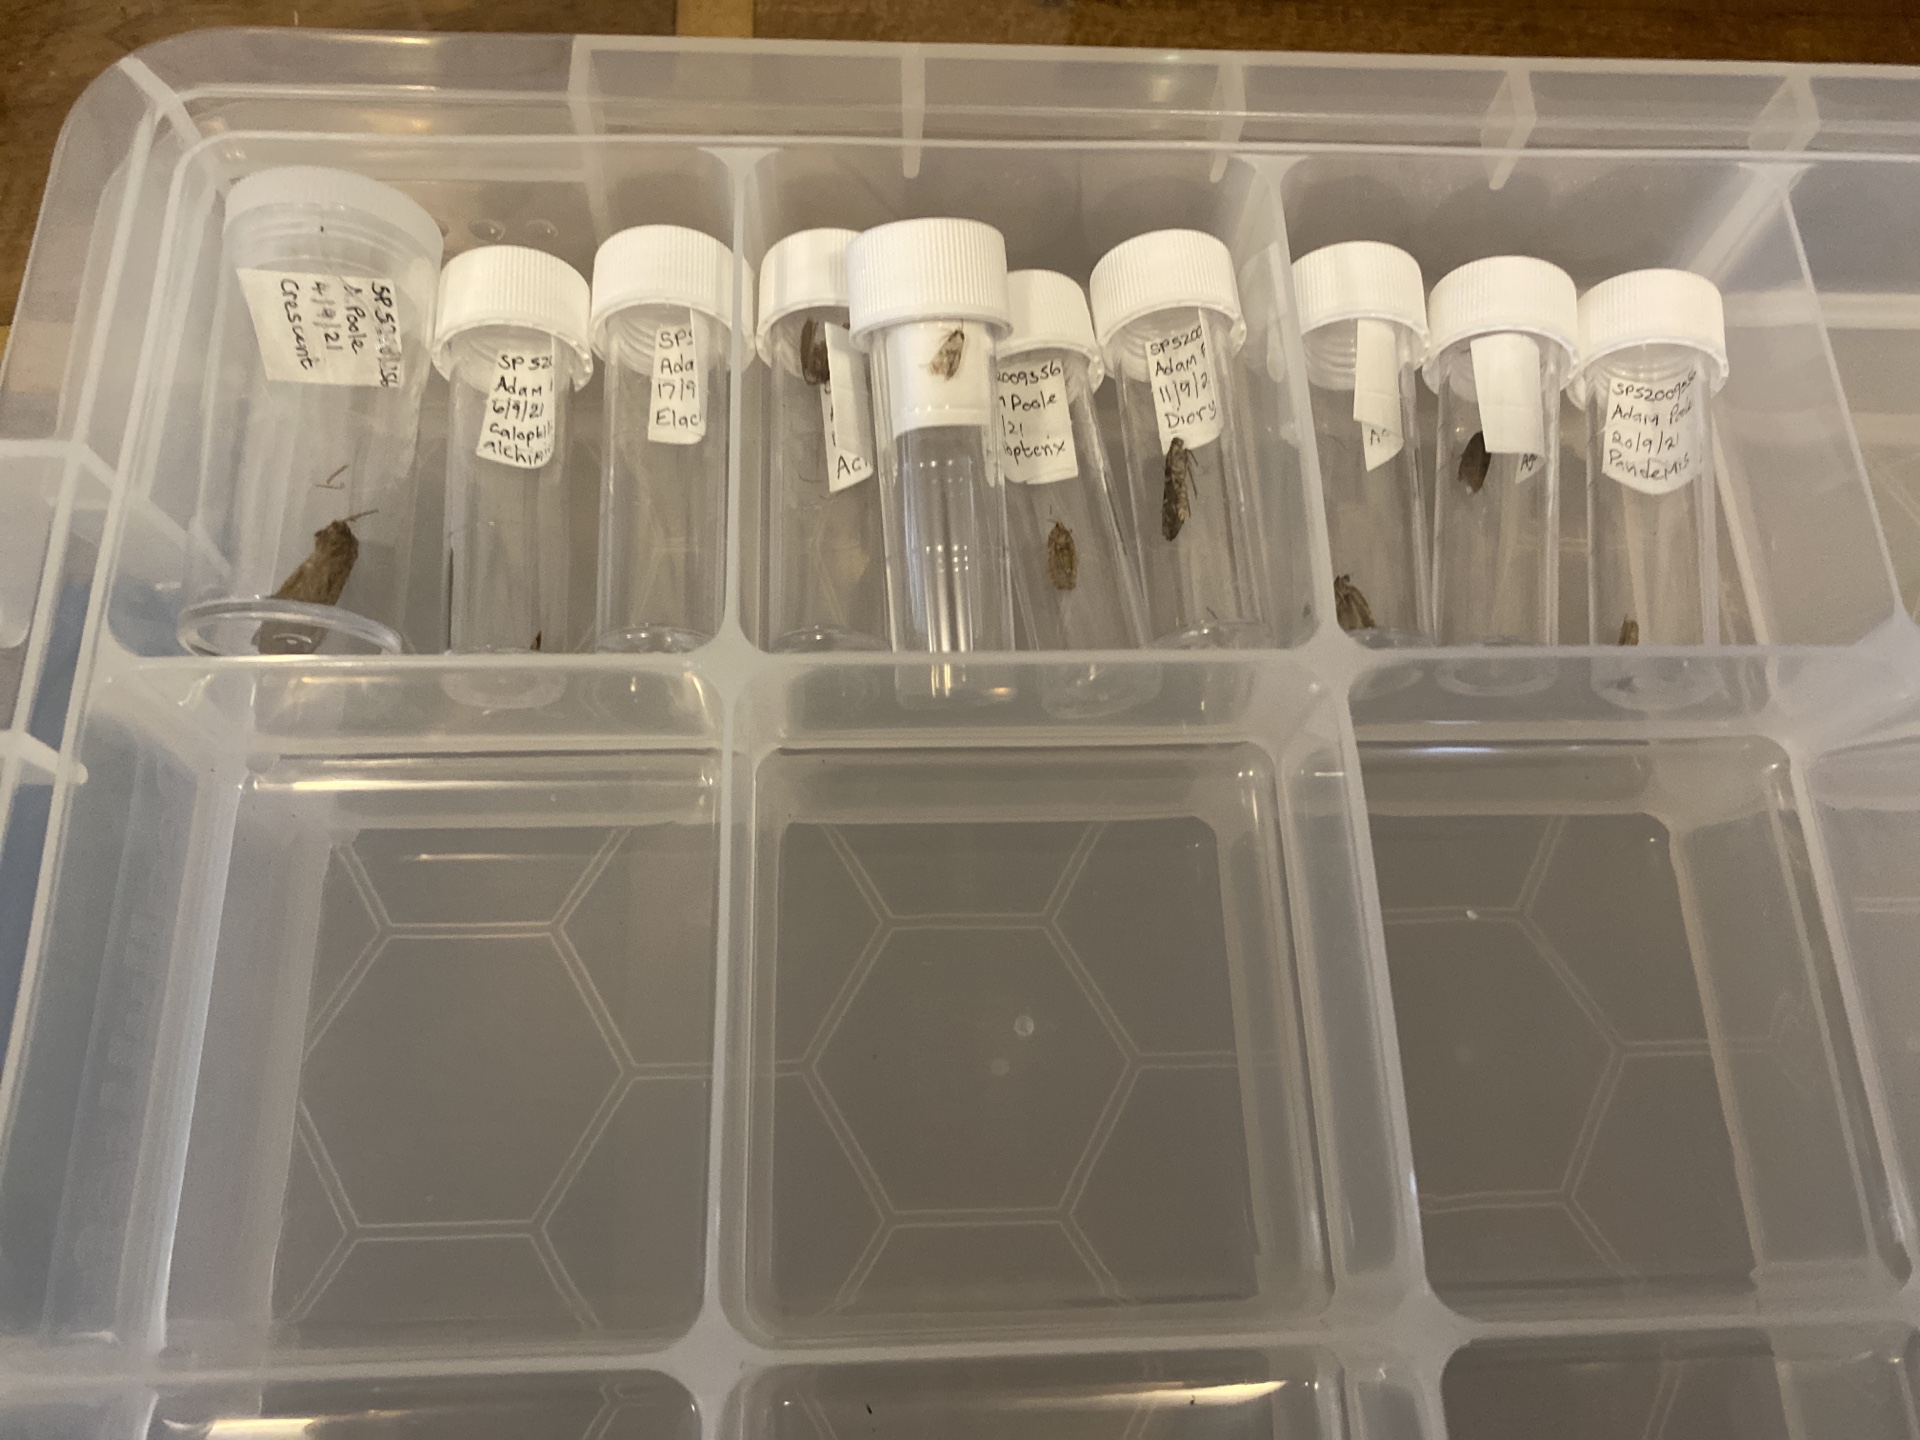
\includegraphics[width=0.3\linewidth]{images/specimens}\hfill
	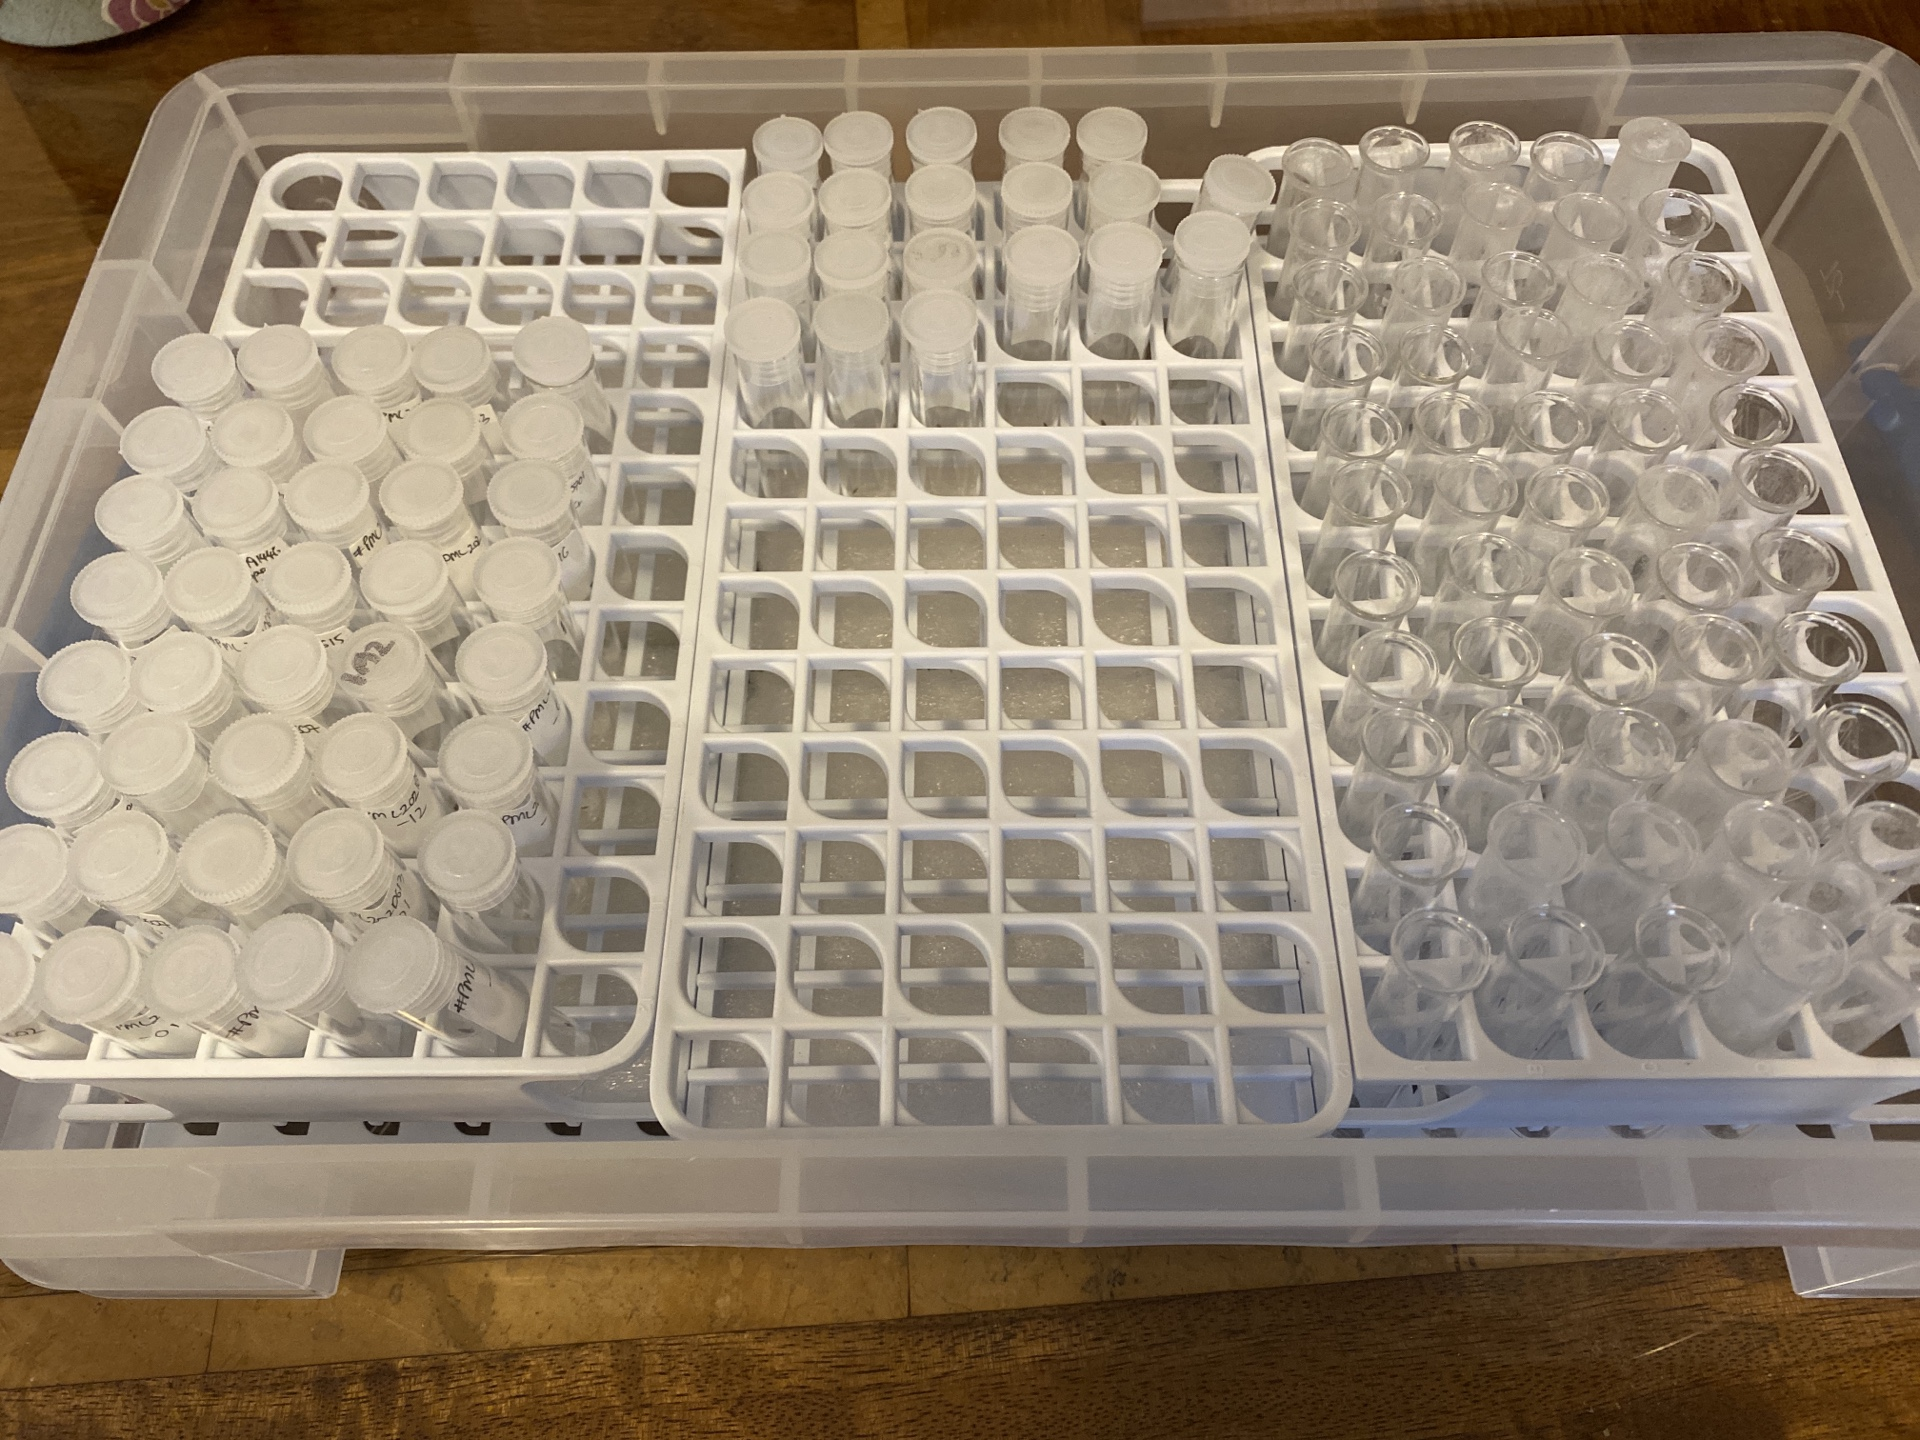
\includegraphics[width=.3\textwidth]{images/prepared}\hfill
	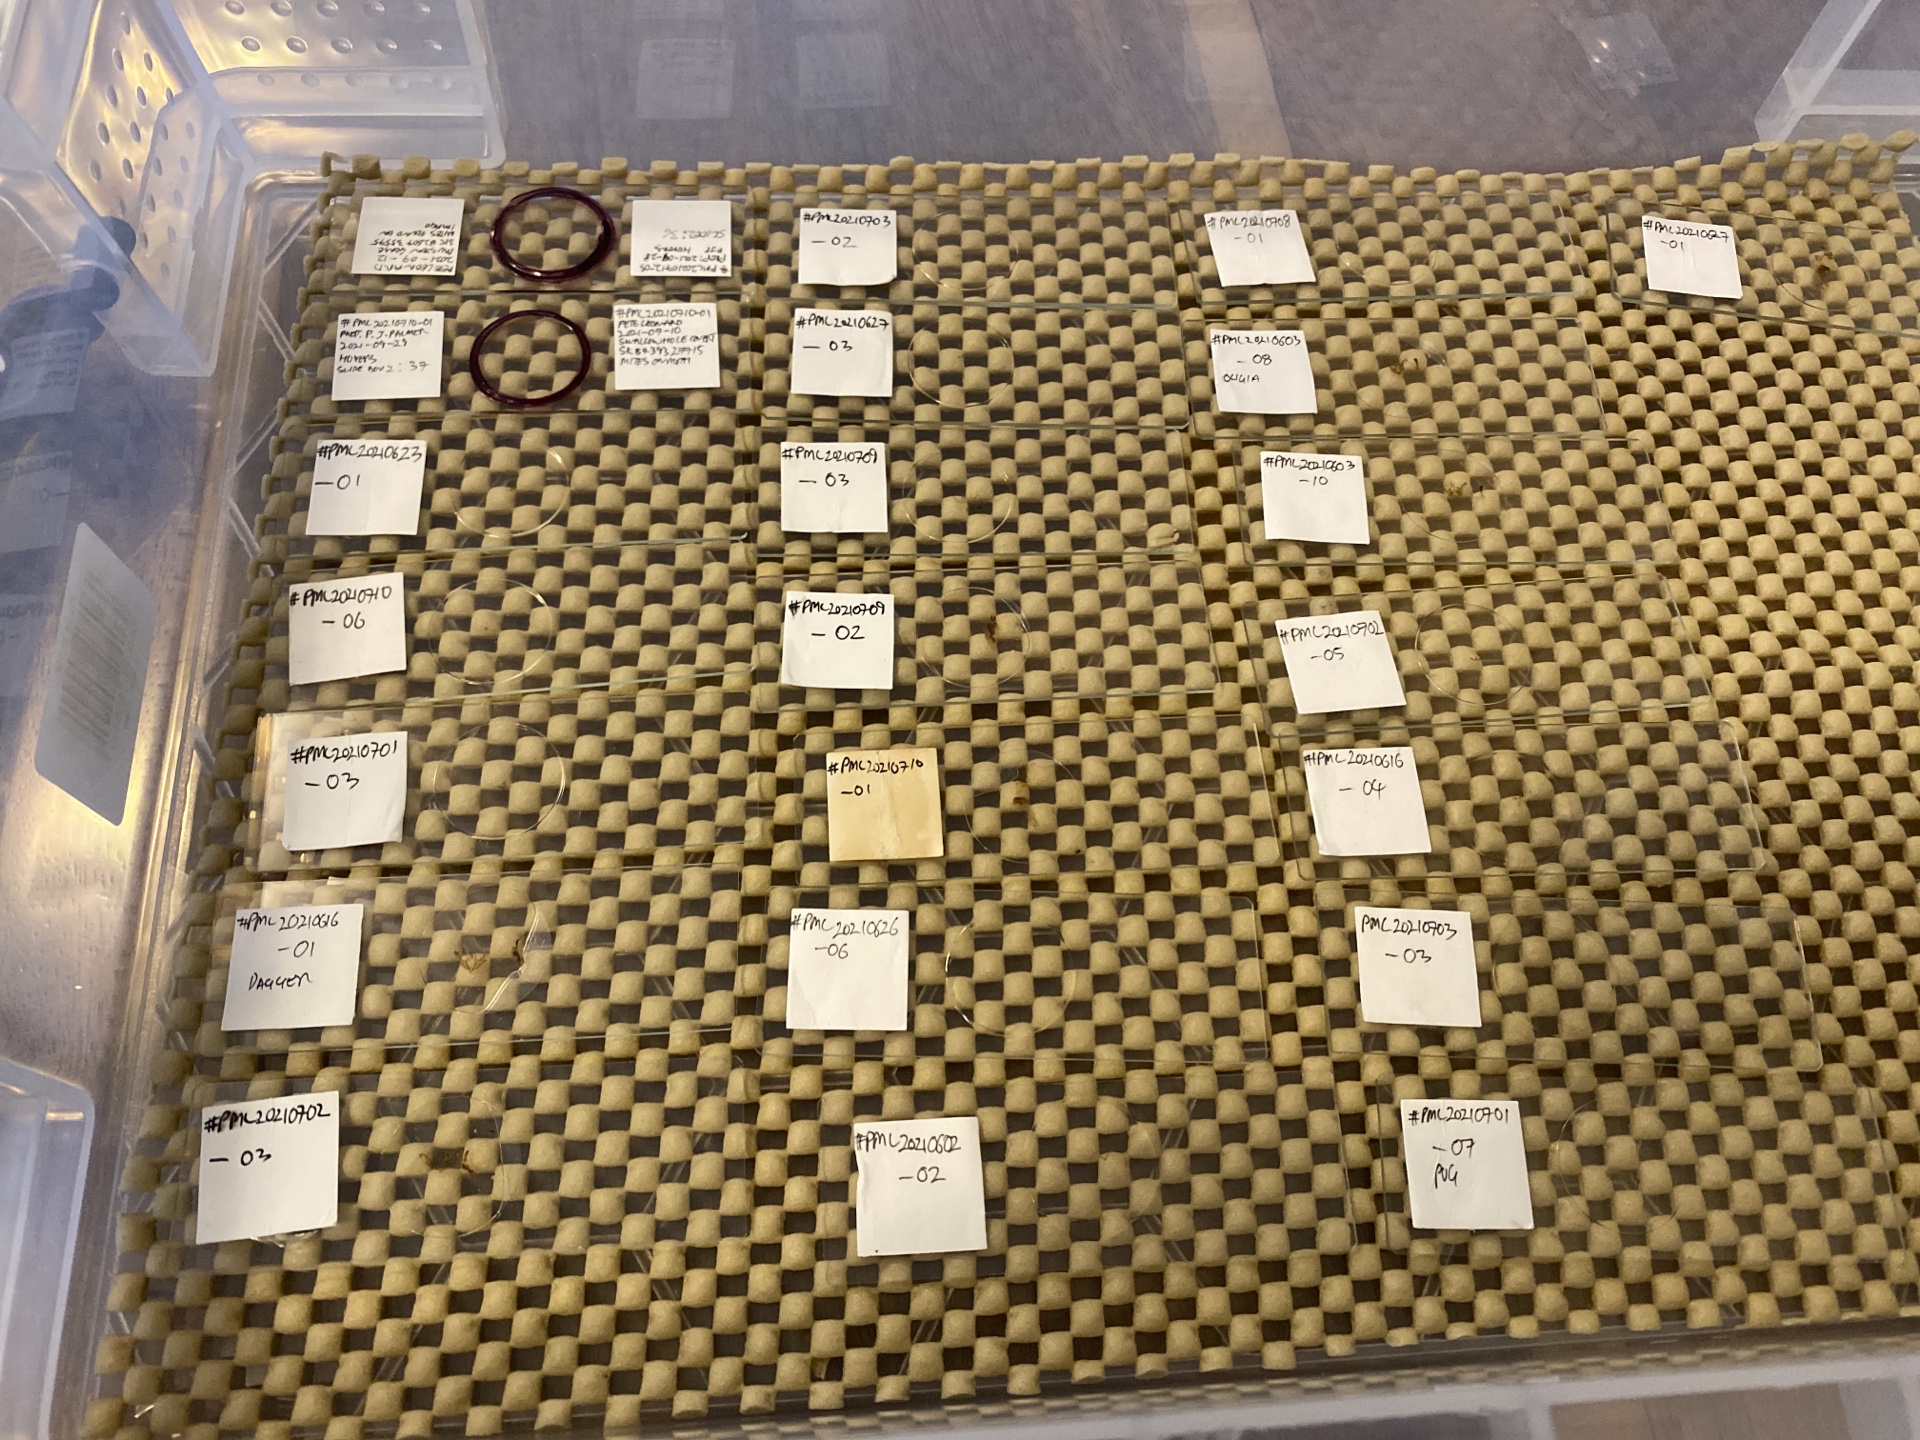
\includegraphics[width=.3\textwidth]{images/slides}\hfill
	\captionof{figure}{From left to right: Specimens as received for examination; Once photographed and catalogued each specimen is placed in a standard tube along with its label; After dissection, the label is glued to the microscope slide.}
	\label{InternalLabel}
\end{center}
Unmounted specimens should be stored in suitable tubes treated in the following way:
\begin{description}

	\item[Label] Create a unique reference number for each specimen. Our suggested format is: your initials, followed by the international date (reverse date) YYYYMMDD, a hyphen, then finally a number for that day (in case there are multiple specimens taken in a day). So the third specimen taken by Paul J. Palmer on 30 April 2022 would become: PJP20220430-03. A label with this number on it should be placed inside the tube along with a single specimen. Figure~\ref{InternalLabel} illustrates how labels are used and why they must be inside the specimen tube. Use a pigment pen or graphite pencil.
	\item[Data] Please complete our simple data spreadsheet, available on request. You need to complete one row per specimen with details such as locality, date and collection method. 
	\item[Photographs] If you are able to take a photograph of the live moth, in a tube if necessary, it can be a very useful aid in the identification process. Please include the unique reference number in the photograph name.
	\item[Freezer] A minimum of 48 hours in a domestic freezer will ensure that the specimen is dead along with any mites that may be present. There is no harm in exceeding this time.
	\item[Dehydration] Exposure to dry air is needed to remove all moisture. An airing cupboard is ideal. The tubes should be uncapped, stoppered with cotton wool, and left for several weeks or longer. 
	\item[Post] The tubes may be posted to: Paul Palmer, 136 Burton Road, Melton Mowbray, Leicestershire LE13 1DL. An advance note is appreciated \\ (\texttt{palmerpjp@gmail.com}) and by arrangement, callers are always welcome.
\end{description}

Please be patient when waiting for results, as we process specimens in batches from multiple recorders which is why we have such specific instructions on labelling and preparation. We will circulate a copy of the report containing your specimens by email when we have identified everything in the batch.


% TODO: \usepackage{graphicx} required





\end{document}
